\documentclass[11pt,a4paper]{article}
\usepackage[margin=24mm]{geometry}
\usepackage{amsmath,amssymb,amsthm,mathtools}
\usepackage{graphicx,booktabs,longtable,array,enumitem,xcolor}
\usepackage{microtype}
\usepackage[colorlinks=true,linkcolor=blue!45!black,urlcolor=blue!45!black,citecolor=blue!45!black]{hyperref}
\usepackage{fancyhdr}
\pagestyle{fancy}\fancyhf{}\fancyhead[L]{HHL logical scaling analysis}\fancyhead[R]{Revision technical report}\fancyfoot[C]{\thepage}
\setlength{\headheight}{14pt}
\makeatletter
\setlength{\@fptop}{0pt}
\setlength{\@fpsep}{18pt}
\setlength{\@fpbot}{0pt plus 1fil}
\makeatother
\setlength{\parskip}{5pt}\setlength{\parindent}{0pt}
\setlist{nosep,leftmargin=*}
\newcommand{\norm}[1]{\left\lVert #1\right\rVert}
\newcommand{\C}{C_{\mathrm{comm}}}
\newcommand{\eps}{\varepsilon}
\newcommand{\HS}{K_{\mathrm{HS1}}}
\newcommand{\ip}{\mathrm{i}}
\newtheorem{theorem}{Theorem}[section]
\newtheorem{lemma}[theorem]{Lemma}
\newtheorem{corollary}[theorem]{Corollary}
\title{HHL Logical Scaling Analysis\\[5pt]\large Corrected derivations, resource accounting, and numerical validation}
\author{HHL paper revision --- Task 03}
\date{9 September 2026}
\begin{document}
\maketitle
\begin{abstract}
This report gives a completed first-order HHL scaling proof for a specified coherent median-QPE and reciprocal-filter circuit. A fixed Trotter microstep defines one Hermitian effective matrix, with a rigorously bounded perturbation obtained from a convergent matrix-logarithm series. Using the same microstep in every controlled power gives a leading one-attempt invocation bound $\widetilde O(L C_{\rm comm}\kappa^2/\varepsilon^2)$, with the lower-order $(1+B)$ term stated in the theorem. Independent repeat-until-success adds a worst-case $O(\kappa^2)$ factor. The theorem explicitly includes QPE confidence, normalized-state error and success probability, while gate and oracle implementations remain costed inputs. The earlier direct-unitary proof is retained as a more conservative alternative. Numerical evidence includes 485 matrices and 3,880 archived evolution measurements, plus new finite checks of the effective-matrix and median-QPE lemmas. The result is a sufficient complexity bound for this construction, not an optimal QLSA result or a physical crossover estimate.
\end{abstract}
\vspace{8pt}
\textbf{Reading guide.} Start with Theorem~\ref{thm:complete} in Section~\ref{sec:complete}: it gives the final analytical scaling and its four-step proof. The later direct-unitary schedule is an alternative, not the final bound. The numerical sections distinguish archived experiments from new validation of the added lemmas. The final resource section separates invocation counts from compiled T-counts and physical costs.

\textbf{Scope.} This revised report consolidates Task 03 and adds the completed theorem. The seven figures reuse archived measurements. Separate new tests check the effective-matrix and median-QPE lemmas; they are reported explicitly in the new proof-validation subsection. Task 01's version 1.0.0 interface is available. Task 02's application handoff was still absent on 9 September 2026, so the Poisson family is a provisional diagnostic, not the agreed final benchmark.
\newpage
\setcounter{tocdepth}{1}
\tableofcontents
\newpage

\section{Problem, notation, and claims under review}
We consider a nonzero right-hand side $b$ and an invertible Hermitian matrix $A\in\mathbb C^{N\times N}$. For the positive-definite specialization, choose a declared scale $\alpha\geq\norm A$ and write $H=A/\alpha$, with spectrum contained in $[1/\kappa_{\mathrm{gap}},1]$. If $\alpha=\norm A$, the tight gap parameter is the spectral condition number $\kappa_2(A)$; a larger normalization generally gives a larger gap parameter. Scalar normalization does not change the spectral condition number itself. Below, $\kappa$ denotes a justified gap parameter when it is used in an inversion success bound.

The ideal state output is
\begin{equation}
 |x\rangle=\frac{H^{-1}|b\rangle}{\norm{H^{-1}|b\rangle}},\qquad |b\rangle=\frac{b}{\norm b}.
\end{equation}
A state output is not a classical solution vector or an arbitrary physical observable. Input preparation, norm recovery and readout require an output-specific model, consistent with the state-oriented HHL setting~\cite{hhl}.

\begin{center}
\begin{tabular}{p{.20\linewidth}p{.72\linewidth}}
\toprule Symbol & Meaning \\\midrule
$N$, $n_{\rm sys}$ & Matrix dimension and $\lceil\log_2 N\rceil$ system-register width.\\
$s$, $L$ & Maximum nonzeros per row and number of Hermitian one-sparse summands; these need not agree.\\
$m$, $b_{\rm bits}$ & Clock-register width and entry/arithmetic precision; both are bit widths, not error tolerances.\\
$\tau_j$, $r_j$ & Evolution time and product-formula step count for clock bit $j$.\\
$\C$, $\Lambda$ & Pair-commutator sum and largest summand norm.\\
$\eta$, $\eps_{\rm PF}$ & Full-circuit implementation error and its allowed normalized-state contribution.\\
$p_{\min}$, $\delta_{\rm rep}$ & Reference-circuit success lower bound and failure allowance for delivering a success.\\
$G_T$, $D$, $Q_{\rm log}$ & T/T$^\dagger$ count, logical dependency depth, and peak live logical qubits.\\
$t_{\rm wall}$ & Physical runtime, in seconds; distinct from evolution time.\\
\bottomrule
\end{tabular}
\end{center}
All matrix norms are spectral norms; vector norms are Euclidean. After dimensionless normalization of $H$, evolution time is also dimensionless. More generally it has inverse units of $H$, and $\tau^2\C$ is dimensionless. No evolution duration below is a hardware runtime.

The supplied manuscript~\cite{manuscript} states a prefactor proportional to
\begin{equation}\label{eq:old}
 \sqrt{\frac{320}{3}}\,\pi\frac{\kappa^2s}{\eps^2}
\end{equation}
for one-sparse invocations, and then multiplies a module gate estimate. Its Appendix B19 asserts an effective-matrix error of the form $|\tau|/r$ on the basis of small numerical samples. A distribution, tail probability, and uniform-in-size theorem are not supplied. We replace that inference; we do not claim to prove the original prefactor.

\section{Completed HHL theorem and final analytical scaling}\label{sec:complete}
\textbf{Correction to the preceding report version.} The earlier report proved a unitary-simulation bound but left general QPE/filter accuracy as an input. Its conditional $\widetilde O(L\C\kappa^3/\eps^3)$ per-attempt estimate is a conservative alternative, not the final scaling below. Here we give a fully specified QPE/filter construction and a stronger consistent-microstep analysis. This recovers a $\kappa^2/\eps^2$ leading dependence \emph{per attempt}, with explicit decomposition and success costs. No empirical extrapolation is used.

\begin{theorem}[Consistent-microstep, first-order HHL]\label{thm:complete}
Let $H=\sum_{a=1}^L H_a$ be Hermitian with spectrum in $[1/\kappa,1]$, $\kappa\geq1$, and let the $H_a$ be Hermitian one-sparse matrices whose controlled exponentials are available as costed primitives. Let $|b\rangle$ be normalized and $0<\eps\leq1/2$. Define
\begin{equation}
 B=\sum_a\norm{H_a},\qquad \C=\sum_{a<b}\norm{[H_a,H_b]}.
\end{equation}
There is an explicitly specified QPE-based reciprocal circuit whose normalized successful joint state is within $\eps$ of $|0_{\rm work}\rangle\otimes|x\rangle$, with $|x\rangle\propto H^{-1}|b\rangle$. With ideal term exponentials and exact reciprocal rotations, its success probability is at least $1/(256\kappa^2)$. It uses
\begin{equation}\label{eq:final-attempt}
 \boxed{\HS^{\rm attempt}=\widetilde O\!\left(
 L\left[\frac{(1+B)\kappa}{\eps}+\frac{\C\kappa^2}{\eps^2}\right]\right)}
\end{equation}
controlled one-sparse exponentials, including inverse QPE. Without amplitude amplification, the expected number per successful state is
\begin{equation}\label{eq:final-success}
 \boxed{\mathbb E\HS^{\rm success}=\widetilde O\!\left(
 L\left[\frac{(1+B)\kappa^3}{\eps}+\frac{\C\kappa^4}{\eps^2}\right]\right).}
\end{equation}
Here $\widetilde O$ suppresses logarithms in $\kappa/\eps$. A cap delivering one success with failure probability at most $\delta$ adds $O(\log(1/\delta))$ to the expected-order budget. These are invocation bounds, not numerical T-counts. State preparation and other gates are counted separately below. No fixed nonzero positions are assumed.
\end{theorem}

\subsection{Step 1: an exact, branch-controlled matrix perturbation}
Set $P(h)=\prod_a e^{\ip H_ah}$ and suppose $0<hB\leq1/2$. Telescoping the product around identity gives
\begin{equation}
 \norm{P(h)-I}\leq\sum_a\norm{e^{\ip H_ah}-I}\leq hB,
 \qquad\norm{e^{\ip Hh}-I}\leq hB.
\end{equation}
For matrices $X,Y$ with norms at most $\rho<1$, the convergent logarithm series and telescoping powers imply
\begin{align}
 \norm{\log(I+X)-\log(I+Y)}
 &\leq\sum_{k=1}^{\infty}\frac{1}{k}\norm{X^k-Y^k}\\
 &\leq\sum_{k=1}^{\infty}\rho^{k-1}\norm{X-Y}
 =\frac{\norm{X-Y}}{1-\rho}.
\end{align}
These are exact convergent-series inequalities. Since $P(h)$ is unitary and stays within distance $1/2$ of identity, its principal logarithm is skew-Hermitian and defines a Hermitian matrix
\begin{equation}
 \widehat H=\frac{\operatorname{Log}P(h)}{\ip h},\qquad
 P(h)=e^{\ip\widehat Hh}.
\end{equation}
Also $\operatorname{Log}(e^{\ip Hh})=\ip Hh$, since $h\norm H\leq1/2$. The first-order local bound proved in Theorem~\ref{thm:pf} now yields
\begin{equation}\label{eq:corrected-matrix}
 \boxed{\norm{\widehat H-H}\leq\frac{2}{h}\norm{P(h)-e^{\ip Hh}}
 \leq h\C.}
\end{equation}
This is the corrected replacement for the original B19-type step. It has a stated branch condition and a decomposition-dependent coefficient; it is not obtained by equating truncated expansions.

Choose $\tau_*=\pi/4$, $d_H=\eps/(16\kappa)$, and
\begin{equation}\label{eq:microstep}
 r_*=\left\lceil\max\left\{1,2B\tau_*,\frac{\C\tau_*}{d_H}\right\}\right\rceil,
 \qquad h=\frac{\tau_*}{r_*}.
\end{equation}
Then $hB\leq1/2$ and $\norm{\widehat H-H}\leq d_H$. Crucially, every QPE power is implemented as
\begin{equation}\label{eq:consistent}
 V^{2^j}=P(h)^{r_*2^j}=e^{\ip\widehat H\tau_*2^j},\qquad V=P(h)^{r_*}.
\end{equation}
Thus all powers are \emph{exact evolutions of the same $\widehat H$}. Independently choosing a different microstep for each power would not justify this argument.

The normalized perturbation lemma proved below gives
\begin{equation}
 \norm{\frac{\widehat H^{-1}b}{\norm{\widehat H^{-1}b}}-
 \frac{H^{-1}b}{\norm{H^{-1}b}}}
 \leq\frac{2\kappa d_H}{1-\kappa d_H}
 =\frac{\eps}{8(1-\eps/16)}<\frac{\eps}{4}.
\end{equation}
Weyl's eigenvalue inequality gives spectrum of $\widehat H$ in $[1/(2\kappa),2]$. Put $J=\widehat H/2$ and $K=4\kappa$. Then $\operatorname{spec}(J)\subseteq[1/K,1]$, its normalized inverse state equals that of $\widehat H$, and $V=e^{\ip\pi J/2}$.

\subsection{Step 2: a specified QPE accuracy and confidence guarantee}
Write $e=\eps/2$, and choose an eigenvalue tolerance and tail probability
\begin{equation}
 d_\lambda=\frac{e}{8K},\qquad \beta=\left(\frac{e}{8K}\right)^2,
 \qquad M=2^m\geq\frac{32}{d_\lambda},
\end{equation}
with $M$ the smallest such power of two. For an eigenvalue $\lambda\in[1/K,1]$ of $J$, QPE on $V$ estimates phase $\phi=\lambda/4$. One $m$-bit QPE register has probabilities
\begin{equation}
 p_k=\left|\frac{1}{M}\sum_{\ell=0}^{M-1}
 e^{2\pi\ip\ell(\phi-k/M)}\right|^2.
\end{equation}
Let $d_k$ be the signed circular phase difference in $[-1/2,1/2]$. Away from $d_k=0$, $|\sin\pi d_k|\geq2|d_k|$ gives
\begin{equation}
 p_k\leq\frac{1}{4M^2d_k^2}.
\end{equation}
For $a=M d_\lambda/4\geq8$, there are at most two outcomes in each unit-width shell of scaled circular distance. Therefore
\begin{equation}
 \Pr(|d_k|>d_\lambda/4)
 \leq\frac12\sum_{n=0}^{\infty}(a+n)^{-2}
 \leq\frac{1}{2(a-1)}\leq\frac1{14}<\frac18.
\end{equation}
Interpret the phase estimate in $[-1/2,1/2)$ and multiply it by four to obtain a signed estimate $z\in[-2,2)$. On the good event this has $|z-\lambda|\leq d_\lambda$; the good interval lies strictly inside the unwrapped phase domain.

Use an odd number $R$ of independent QPE registers conditional on each eigenstate, with
\begin{equation}
 R\geq\frac{32}{9}\log\frac1\beta,
\end{equation}
and compute the median of their signed estimates reversibly. If a majority are good, the median is good. For Bernoulli failures of mean at most $1/8$, the exponential-moment (Hoeffding) bound gives
\begin{equation}
 \Pr(\text{at least }R/2\text{ failures})
 \leq\exp[-2R(1/2-1/8)^2]=e^{-9R/32}\leq\beta.
\end{equation}
For completeness, the exponential-moment step uses $\mathbb E e^{t(X-\mathbb EX)}\leq e^{t^2/8}$ for $X\in[0,1]$, followed by independence, Markov's inequality, and minimization in $t$. The moment inequality itself follows because the second derivative of the log moment-generating function is a tilted variance, at most $1/4$ for a variable in $[0,1]$, and its centered value and first derivative vanish at zero. Conditional eigenstate probabilities are independent even though the overall algorithm is coherent on a superposition of eigenstates.

\subsection{Step 3: reciprocal filter, uncomputation, and success}
On the median register use the bounded success amplitude
\begin{equation}
 f(z)=\frac{c}{\max\{z,1/(2K)\}},\qquad c=\frac1{2K}.
\end{equation}
It lies in $[0,1]$ for every signed estimate, including negative and near-zero values. Uncompute the median and all QPE registers after the controlled rotation. Let $a_0$ denote the hypothetical successful vector obtained with the exact function $c/\lambda$. It equals $|0_{\rm work}\rangle\otimes cJ^{-1}|b\rangle$, and
\begin{equation}
 p_0=\norm{a_0}^2=c^2\norm{J^{-1}b}^2\geq\frac1{4K^2}.
\end{equation}
On a good estimate, $z\geq\lambda-d_\lambda\geq\lambda/2\geq1/(2K)$, so
\begin{equation}
 |f(z)-c/\lambda|\leq 2K d_\lambda\,(c/\lambda).
\end{equation}
On the bad event the absolute difference is at most one. Squaring and averaging for each eigenstate, then summing over the orthogonal system eigenstates, gives for the actual successful vector $a$
\begin{equation}
 \norm{a-a_0}\leq2K d_\lambda\sqrt{p_0}+\sqrt\beta.
\end{equation}
Uncomputing the registers preserves this distance. Normalization hence gives
\begin{align}
 \norm{a/\norm a-a_0/\norm{a_0}}
 &\leq4K d_\lambda+\frac{2\sqrt\beta}{\sqrt{p_0}}\\
 &\leq4K d_\lambda+4K\sqrt\beta=e.
\end{align}
Moreover
\begin{equation}
 \norm a\geq\sqrt{p_0}(1-2K d_\lambda-2K\sqrt\beta)
 =\sqrt{p_0}(1-e/2),\qquad
 p=\norm a^2\geq\frac1{16K^2}=\frac1{256\kappa^2}.
\end{equation}
Adding the $<\eps/4$ matrix-perturbation contribution to $e=\eps/2$ proves error less than $3\eps/4$ and leaves margin for gate implementation.

If the implemented attempted circuit differs from this reference by operator norm at most $\eta_{\rm impl}=\eps/(64K)$, the normalization bound adds at most $8K\eta_{\rm impl}=\eps/8$. Success remains at least $1/(25K^2)=1/(400\kappa^2)$. Thus synthesis, entry and arithmetic approximations can be budgeted explicitly while retaining error below $\eps$ and the same polynomial scaling. This is a precision requirement, not an assertion that the repository's fixed precision already meets it.

\subsection{Step 4: counting the circuit and its repetitions}
Each of the $R$ QPE registers uses $r_*(M-1)$ applications of the microstep $P(h)$, since $\sum_{j=0}^{m-1}2^j=M-1$. Each microstep uses $L$ controlled term exponentials. Inverse QPE doubles this:
\begin{equation}\label{eq:exact-newcount}
 \boxed{\HS^{\rm attempt}=2LRr_*(M-1).}
\end{equation}
Here $R=O(\log(\kappa/\eps))$, $M=O(\kappa/\eps)$ and
$r_*=O(1+B+\C\kappa/\eps)$. Substitution proves equation~\eqref{eq:final-attempt}. Multiplication by $O(\kappa^2)$ expected independent attempts proves equation~\eqref{eq:final-success}. A sufficient implemented-circuit delivery cap is $\lceil400\kappa^2\log(1/\delta)\rceil$, using $(1-p)^r\leq e^{-pr}$.

If $g_{\rm HS1}$ is a valid compiled T-count upper bound per controlled term, and $G_{\rm prep},G_{\rm other}$ are the remaining per-attempt T-counts, the resource statement is
\begin{equation}\label{eq:final-gates}
 \boxed{\mathbb E G_T^{\rm success}
 \leq 400\kappa^2\left(G_{\rm prep}+G_{\rm other}
       +g_{\rm HS1}\,\HS^{\rm attempt}\right).}
\end{equation}
The constant 400 uses the implementation allowance above; it is a conservative bound. $G_{\rm other}$ includes all QFTs, reversible median computation, reciprocal rotation, and heralding/control logic, under an exclusive gate convention. Oracle implementations and their uncomputation are included in $g_{\rm HS1}$ or charged separately, never omitted.

One explicit finite implementation of the reciprocal uses a classical table of the $M$ possible median values and one controlled rotation per value. With multi-controlled operations decomposed using workspace, this requires $O(Mm)$ elementary controlled logic plus $M$ synthesized rotations, and classical angle-table construction. A reversible comparison-sort network for the median uses at most $O(R^2m)$ elementary operations; QFTs contribute $O(Rm^2)$ rotations/controlled gates. With the separately specified rotation-synthesis overhead included~\cite{synthesis}, these bounds make the non-HS overhead polynomial and explicit; they do not identify an optimal arithmetic implementation. Classical preprocessing and input preparation remain charged resources. Clock storage is $Rm$, not the single $m$-bit register of the earlier demonstration.

\subsection{What this means for sparsity and the old claim}
For the disjoint-entry greedy coloring construction, $L\leq2s$, $B\leq L$, and $\C\leq L(L-1)$. A conservative general sparse consequence is
\begin{equation}
 \HS^{\rm attempt}=\widetilde O(s^3\kappa^2/\eps^2),\qquad
 \mathbb E\HS^{\rm success}=\widetilde O(s^3\kappa^4/\eps^2).
\end{equation}
These are upper bounds for this construction, not optimal QLSA complexities. For a structured family with $L=O(s)$ and a genuinely proved $\C=O(1)$, the leading per-attempt term is instead $\widetilde O(s\kappa^2/\eps^2)$, provided the $(1+B)\kappa/\eps$ term does not dominate. This is the restricted circumstance in which the earlier leading dependence can be recovered. It cannot be claimed for arbitrary sparse matrices merely by inspecting small samples.

No amplitude amplification is included in this theorem. If a different implementation uses it, its coherent circuit and success accounting must replace the independent-retry model. Nor are the old prefactor $\sqrt{320/3}\pi$, a free fixed-position oracle, or a numerical hardware crossover established by this proof. The previously reported direct-unitary schedule remains a valid alternative; its example count 417852 and archived HHL figures are not measurements of the new median-QPE construction.

\subsection{Explicit constants and validation status}
The accompanying \texttt{completed\_schedule.py} evaluates all integer choices. For example, scale the archived two-dimensional test by $4/3$ so its spectrum is $[1/3,1]$. Its parameters are $L=3$, $B=17/15$, $\C=8/75$. At $\eps=0.25$, the theorem chooses $r_*=17$, $m=15$, $R=49$, and 163769466 controlled term invocations per attempt. This large sufficient count illustrates the conservatism of the explicit confidence and error constants. It is neither a measured requirement nor an optimized implementation, and cannot replace the old resource prefactor as an equally tight practical estimate.

The logarithm, perturbation, and median-QPE lemmas are tested separately in the new validation subsection. The seven archived figures continue to describe their original circuits and matrix ensembles; they are not presented as a full simulation of the new coherent median-QPE circuit.


\section{A deterministic product-formula bound}
\subsection{Two-term local error}
Let $A_1,A_2$ be Hermitian and $V(t)=e^{\ip A_1t}e^{\ip A_2t}$, $U(t)=e^{\ip(A_1+A_2)t}$. Direct differentiation gives
\begin{align}
 V'(t)&=\ip(A_1+A_2)V(t)+R(t),\\
 R(t)&=\left(e^{\ip A_1t}\ip A_2e^{-\ip A_1t}-\ip A_2\right)V(t).
\end{align}
The conjugation difference has the exact representation
\begin{equation}
 e^{\ip A_1t}\ip A_2e^{-\ip A_1t}-\ip A_2
 =\int_0^t e^{\ip A_1v}[\ip A_1,\ip A_2]e^{-\ip A_1v}\,dv.
\end{equation}
For $t\geq0$, unitary invariance implies $\norm{R(t)}\leq t\norm{[A_1,A_2]}$. Variation of parameters yields
\begin{equation}
 V(t)-U(t)=\int_0^t U(t-u)R(u)\,du,
\end{equation}
so
\begin{equation}\label{eq:two}
 \norm{V(t)-U(t)}\leq\frac{t^2}{2}\norm{[A_1,A_2]}.
\end{equation}
For negative $t$, apply the same proof to $-A_1,-A_2$. This is an exact integral estimate; it does not discard a Taylor or Dyson remainder. The two-term result and its grouped multi-term counterpart appear in Childs et al., Proposition 15~\cite{trotter}.

\subsection{Many terms and repeated steps}
Write
\begin{equation}
 H=\sum_{a=1}^L H_a,\quad P(t)=\prod_{a=1}^L e^{\ip H_at},\quad
 \C=\sum_{1\leq a<b\leq L}\norm{[H_a,H_b]}.
\end{equation}
The displayed product fixes one ordering; the same pairwise bound applies to any ordering. Successively split the first summand from the remaining sum. At split $a$, equation~\eqref{eq:two} contributes at most
\begin{equation}
 \frac{t^2}{2}\norm{\left[H_a,\sum_{b>a}H_b\right]}
 \leq\frac{t^2}{2}\sum_{b>a}\norm{[H_a,H_b]}.
\end{equation}
Telescoping these splits, with unitary factors of norm one, proves $\norm{P(t)-e^{\ip Ht}}\leq t^2\C/2$.

For any unitaries $V,W$ and positive integer $r$,
\begin{equation}
 V^r-W^r=\sum_{k=0}^{r-1}V^{r-1-k}(V-W)W^k,
 \qquad \norm{V^r-W^r}\leq r\norm{V-W}.
\end{equation}
Set $V=P(\tau/r)$ and $W=e^{\ip H\tau/r}$ to obtain the central result.

\begin{theorem}[First-order simulation guarantee]\label{thm:pf}
For any finite-dimensional Hermitian decomposition and $r\geq1$,
\begin{equation}\boxed{
 \norm{S_r(\tau)-e^{\ip H\tau}}\leq
 \min\left\{2,\frac{\tau^2\C}{2r}\right\},\qquad
 S_r(\tau)=\left(\prod_{a=1}^L e^{\ip H_a\tau/r}\right)^r.}
\end{equation}
\end{theorem}
The ceiling two follows independently from the triangle inequality for two unitaries. There is no probabilistic qualifier and no assumption about positions of nonzero entries.

\subsection{What dimension independence actually requires}
By submultiplicativity,
\begin{equation}\label{eq:envelope}
 \C\leq2\sum_{a<b}\norm{H_a}\norm{H_b}
 \leq L(L-1)\Lambda^2,\qquad \Lambda=\max_a\norm{H_a}.
\end{equation}
Thus families with uniformly bounded $L$ and $\Lambda$ have a dimension-uniform simulation coefficient at fixed $\tau,r$. This is a sufficient restricted result. It does not imply that the measured error is constant, or that the full HHL cost is independent of $N$. Evolution times, gap, access costs and precision can all grow. Normalization $\norm H=1$ alone does not bound the summand norms because terms can cancel.

\subsection{Removing fixed matrix-element positions}
A generic existence construction for a real symmetric $s$-sparse matrix uses an undirected graph for its off-diagonal nonzeros. If its maximum degree is $\Delta\geq1$, any edge conflicts with at most $2\Delta-2$ other incident edges. Greedy edge coloring therefore uses at most $2\Delta-1$ colors. Each color is a matching, and its weighted adjacency matrix is Hermitian one-sparse. A separate diagonal term is also one-sparse. Hence
\begin{equation}
 L\leq2\Delta\leq2s,
\end{equation}
with absent terms omitted; a purely diagonal matrix needs one term. For a matching term its norm is the largest absolute edge weight, since every nonzero block has eigenvalues $\pm|w|$. With $\alpha\geq\norm A$, $|A_{ij}|/\alpha\leq1$, so $\Lambda\leq1$ for this disjoint-entry construction.

This is an existence and classical preprocessing statement, not a free coherent oracle. A direct greedy implementation can use $O(Ns^2)$ work and $O(Ns)$ edge storage, followed by separately costed lookup and compilation. The repository's implicit coloring routine instead enumerates $6s^2$ terms. Its access implementation and correctness are separate inputs. Complex Hermitian matching blocks permit conjugate edge weights, but the real-valued module gate estimate does not automatically transfer to them.

\section{Effective-Hamiltonian errors and normalization}
\subsection{Why the original exponential argument fails}
The original B5 is a time-ordered exponential. B6 and B7 truncate Dyson and Taylor expansions, then B8 treats their first-order match as an exact identity for $H'-H$. The omitted terms are not zero. Consequently the first equality used in B18 is unproved.

Moreover, a unitary logarithm is nonunique. Even with an exact evolution, the principal expression
\begin{equation}
 H_{\rm eff}(\tau)=\frac{\operatorname{Log}(e^{\ip H\tau})}{\ip\tau}
\end{equation}
need not equal $H$ when eigenphases wrap. A small unitary error at one time does not alone certify a matrix perturbation or one common perturbed matrix across independently approximated QPE powers. Section~\ref{sec:complete} supplies a sufficient branch condition and an exact logarithm-series bound. The explicit small-phase diagnostics below illustrate why an unrestricted use of the logarithm was invalid.

\subsection{An analytic check of the original two-term example}
Let $X,Y,Z$ be the Pauli matrices, $c=\cos\tau$, $s_\tau=\sin\tau$, and $U=e^{\ip Z\tau}e^{\ip X\tau}$. Using $ZX=\ip Y$,
\begin{equation}
 U=c^2I+\ip\big[c s_\tau(X+Z)-s_\tau^2Y\big].
\end{equation}
On the branch continuously connected to $\tau=0$, put $\theta=\arccos(c^2)$. Then
\begin{align}
 H_{\rm eff}&=\frac{\theta}{\tau\sin\theta}
       \big[c s_\tau(X+Z)-s_\tau^2Y\big],\\
 \norm{H_{\rm eff}-(X+Z)}
 &=\sqrt{2\left(\frac{\theta c s_\tau}{\tau\sin\theta}-1\right)^2
        +\left(\frac{\theta s_\tau^2}{\tau\sin\theta}\right)^2}.
\end{align}
At $\tau=0.2$ the archived numerical value is $0.2008868159$, whereas B18's written right-hand side is $0.2$, not $0.1$. At $\tau=0.1$ the error is $0.1001110486$ versus $0.1$. The old finite-time equality is false. The corresponding unitary errors, $0.0396458835$ and $0.0099778003$, satisfy Theorem~\ref{thm:pf}, whose bounds here are $\tau^2$.

A second stress test uses the one-sparse terms $2Z,2X,-2Z,-2X,I$. Their sum is the normalized SPD matrix $I$. For $\tau=0.001,r=1$, the effective-matrix error is $0.0079999893>|\tau|$. The group commutator has leading term $-\tau^2[2Z,2X]=-8\ip\tau^2Y$, explaining an effective error of order $8|\tau|$. This refutes a decomposition-independent reading of B19. It is a cancelling decomposition, not a disjoint-entry coloring example.

\subsection{The valid matrix-perturbation lemma}
For completeness, if $x=A^{-1}b$, $y=(A+E)^{-1}b$, and $q=\norm{A^{-1}}\norm E<1$, the Neumann bound gives
\begin{align}
 y-x&=-(I+A^{-1}E)^{-1}A^{-1}Ex,\\
 \frac{\norm{y-x}}{\norm x}&\leq\frac{q}{1-q}.
\end{align}
For nonzero $x,y$, adding and subtracting $y/\norm x$ and using the reverse triangle inequality gives
\begin{equation}\label{eq:normalize}
 \norm{\frac{y}{\norm y}-\frac{x}{\norm x}}
 \leq\frac{2\norm{y-x}}{\norm x}
 \leq\frac{2q}{1-q}.
\end{equation}
The original B20 concerns unnormalized solutions; B21 cannot simply impose $\norm x=1$ while retaining the same fixed normalized right-hand side. The corrected lemma still requires a valid matrix-perturbation premise, which B19 did not establish. We instead propagate circuit error directly.

\section{From controlled evolutions to a successful HHL state}
\subsection{Phase estimation and its inverse}
For $m$ clock bits let $\tau_j=\tau_{\rm base}2^j$, $0\leq j<m$, and approximate each controlled evolution using $r_j$ product steps. The difference between controlled unitaries is block diagonal with blocks zero and the underlying difference; its norm is unchanged. Adjointing also preserves the norm.

For products of unitary circuit blocks, telescoping bounds the total difference by the sum of block differences. Including forward and inverse QPE therefore gives
\begin{equation}\label{eq:circuit}
 \boxed{\eta_{\rm PF}\leq
 2\sum_{j=0}^{m-1}\frac{\tau_j^2\C}{2r_j}
 =\C\sum_{j=0}^{m-1}\frac{\tau_j^2}{r_j}.}
\end{equation}
This is a full premeasurement circuit bound. It is neither a normalized successful-state error nor a proof of finite-QPE inversion accuracy.

For reference, on an exact eigenstate with phase $\phi=\lambda\tau_{\rm base}/(2\pi)$, uniform-clock QPE produces amplitudes
\begin{equation}
 a_k(\phi)=\frac{1}{M}\sum_{\ell=0}^{M-1}
 e^{2\pi\ip\ell(\phi-k/M)},\qquad M=2^m.
\end{equation}
Only when $\phi=k_0/M$ is this exactly supported at one bin $k_0$. Otherwise tails encounter the reciprocal filter, including its behavior near zero. Choosing $m$ by itself does not certify a bound on the resulting inverse state. A general guarantee must specify spectral range, alias avoidance, signed-phase handling where needed, cutoff, reciprocal approximation and tail control. The exact-grid test in the tractable validation section deliberately avoids inferring such a theorem.

\subsection{Postselection and success probability}
Let $U$ be the reference circuit with exact evolutions, $\widetilde U$ its implementation, and $P$ the projector onto the successful flag. For a normalized initial state $|\psi\rangle$, define
\begin{equation}
 a=PU|\psi\rangle,\qquad \widetilde a=P\widetilde U|\psi\rangle,
 \qquad p=\norm a^2\geq p_{\min}>0.
\end{equation}
If $\norm{\widetilde U-U}\leq\eta$, then projection is contractive and $\norm{\widetilde a-a}\leq\eta$. Equation~\eqref{eq:normalize} gives
\begin{equation}\label{eq:post}
 \boxed{\norm{\frac{\widetilde a}{\norm{\widetilde a}}-\frac{a}{\norm a}}
 \leq\frac{2\eta}{\sqrt{p_{\min}}}.}
\end{equation}
The reverse triangle inequality further yields, when $\eta<\sqrt{p_{\min}}$,
\begin{equation}\label{eq:success}
 p_{\rm implemented}=\norm{\widetilde a}^2
 \geq(\sqrt{p_{\min}}-\eta)^2.
\end{equation}
The state bound applies to the whole successful clock/system branch. Partial trace cannot increase trace distance. For an allowed PF contribution $\eps_{\rm PF}<1$, it suffices to choose
\begin{equation}\label{eq:budget}
 \eta_{\rm target}=\frac{\eps_{\rm PF}\sqrt{p_{\min}}}{2},
 \qquad \eta_{\rm PF}\leq\eta_{\rm target}.
\end{equation}

Reference algorithm error and implementation error are distinct. If the reference successful state is within $\eps_{\rm ref}$ of the target, their joint bound is $\eps_{\rm ref}+2\eta/\sqrt{p_{\min}}$. Entry, synthesis, arithmetic and other full-circuit errors must be included in $\eta$ before using equation~\eqref{eq:success} as a final delivery guarantee.

\subsection{Exact inversion and repetitions}
With exact reciprocal rotation amplitude $c/\lambda$, the ideal successful branch is $cH^{-1}|b\rangle$ and
\begin{equation}
 p=c^2\norm{H^{-1}|b\rangle}^2.
\end{equation}
For spectrum in $[1/\kappa,1]$ and $c=1/\kappa$, one has $p\geq\kappa^{-2}$. This premise is exact inversion; a finite-clock/filter circuit requires its own success certificate.

Independent repeat-until-success uses expected attempts $1/p_{\rm implemented}$. With a valid $0<p_{\rm lower}<1$, a sufficient cap for failure probability $\delta_{\rm rep}\in(0,1)$ is
\begin{equation}\label{eq:reps}
 R_{\rm cap}=\left\lceil\frac{\log\delta_{\rm rep}}{\log(1-p_{\rm lower})}\right\rceil,
 \qquad \Pr(\text{no success})\leq(1-p_{\rm lower})^{R_{\rm cap}}.
\end{equation}
If $p_{\rm lower}=1$, one attempt suffices. An expected count is not a delivery cap. Preparing many successful samples for an observable adds another explicitly owned multiplicity. Amplitude amplification requires a different coherent circuit; its square-root success improvement cannot be inserted into the current schedule without modeling that circuit.

\section{Alternative direct-unitary logical-resource schedule}
This section retains the earlier independent-power error-allocation method. Its conditional asymptotic estimate is looser than Theorem~\ref{thm:complete}; it is not the final analytical scaling. Its archived numerical adapter and examples are retained for traceability.
\subsection{Step allocation and its derivation}
Let $S=\sum_j|\tau_j|$. To minimize the continuous proxy $\sum_jr_j$ under equation~\eqref{eq:circuit}, Cauchy--Schwarz gives
\begin{equation}
 S^2=\left(\sum_j\sqrt{r_j}\frac{|\tau_j|}{\sqrt{r_j}}\right)^2
 \leq\left(\sum_jr_j\right)\left(\sum_j\frac{\tau_j^2}{r_j}\right).
\end{equation}
Equality requires $r_j\propto|\tau_j|$. This optimizes this bound-based continuous proxy, not the true gate-optimal simulation. A valid integer choice for $\C>0$ is
\begin{equation}\label{eq:schedule}
 \boxed{r_j=\max\left\{1,\left\lceil\frac{\C S|\tau_j|}{\eta_{\rm target}}\right\rceil\right\}.}
\end{equation}
Each summand in equation~\eqref{eq:circuit} is then at most $\eta_{\rm target}|\tau_j|/S$, so the target holds. For $\C=0$, take every $r_j=1$.

Each step uses $L$ controlled one-sparse exponentials. Including inverse QPE gives
\begin{equation}\label{eq:count}
 \boxed{\HS=2L\sum_jr_j\leq2L\left(m+\frac{\C S^2}{\eta_{\rm target}}\right).}
\end{equation}
For the powers-of-two clock, $S=|\tau_{\rm base}|(2^m-1)$. The count does not merge adjacent factors. If term or clock-dependent costs differ, the weighted objective should replace $\sum_jr_j$; the displayed schedule remains sufficient without claiming weighted optimality.

\subsection{From term invocations to gates, depth, and space}
Let $g_{a,j}$ and $\bar g_{a,j}$ be compiled forward and inverse controlled-term counts in an exclusive primitive gate bucket. The attempted-circuit cost is
\begin{align}
 G_{\rm attempt}={}&G_{\rm prep}+G_{\rm QPE,nonHS}+G_{\rm recip}
 +G_{\rm inverseQPE,nonHS}+G_{\rm herald}\nonumber\\
 &+\sum_jr_j\sum_a(g_{a,j}+\bar g_{a,j}).
\end{align}
Term costs must include controls, color/position/value access, uncomputation and synthesis. A homogeneous bound $g_{a,j},\bar g_{a,j}\leq g_{\rm HS1}$ gives simulation cost at most $\HS g_{\rm HS1}$. A module's unexpanded oracle-query count cannot be treated as an implemented T-count.

Serial logical depth is a sum of dependency depths, and T-depth is the corresponding scheduled non-Clifford depth; neither equals gate count in general. Peak logical space is
\begin{equation}
 Q_{\rm log,peak}=n_{\rm sys}+m+1+W_{\rm peak},
\end{equation}
where $W_{\rm peak}$ covers simultaneously live extra workspace for the actual schedule. Preparation and readout can raise this peak. Workspace from disjoint phases should not simply be summed, while retained registers must remain counted.

If a Hermitian entry approximation produces $H+E$, Duhamel's formula gives
\begin{align}
 e^{\ip(H+E)\tau}-e^{\ip H\tau}
 &=\ip\int_0^\tau e^{\ip(H+E)(\tau-u)}E e^{\ip Hu}\,du,\\
 \norm{e^{\ip(H+E)\tau}-e^{\ip H\tau}}&\leq|\tau|\norm E.
\end{align}
If each row has at most $s$ affected entries of magnitude at most $\delta_a$ and $E$ is Hermitian, $\norm E\leq\sqrt{\norm E_1\norm E_\infty}\leq s\delta_a$. This conditional entry-precision bound must be summed over both QPE directions and combined with the other error budgets. Synthesis errors similarly accumulate over the actual implemented gates. No fixed $b_{\rm bits}$ is automatically adequate for every size and tolerance.

\subsection{Conditional asymptotic dependence}
Suppose a separately certified QPE/filter family has $S=O(\kappa/\eps_{\rm QPE})$ and $p_{\min}=\Omega(\kappa^{-2})$. Equations~\eqref{eq:budget} and~\eqref{eq:count} yield the sufficient per-attempt bound
\begin{equation}\label{eq:conditional}
 \HS=O\left(Lm+
 \frac{L\C\kappa^3}{\eps_{\rm QPE}^2\eps_{\rm PF}}\right).
\end{equation}
With comparable error budgets this is $O(Lm+L\C\kappa^3/\eps_{\rm state}^3)$. For fixed small implementation error relative to $\sqrt{p_{\min}}$, repeats can add $O(\kappa^2)$ in expectation, or a factor with $\log(1/\delta_{\rm rep})$ for capped delivery. Gate costs multiply these invocation counts.

This is a conservative consequence of the chosen proof and scheduling strategy. It is not an optimal HHL theorem, a lower bound, or evidence that a quantum advantage is impossible. In particular it does not validate equation~\eqref{eq:old}. Combining the crude envelope $\C\leq L(L-1)\Lambda^2$ introduces up to cubic dependence on $L$ in the simulation count; replacing $L$ changes both per-step work and the error coefficient. A universal extra factor such as the manuscript's $60s$ is not a complete repair.

\section{Structured Poisson family and conditioning}
\subsection{Discretization and spectrum}
On $(0,1)^2$, consider $-\Delta u=f$ with zero Dirichlet boundary conditions. Use $q$ interior points per side, $h=1/(q+1)$ and $N=q^2$. The five-point discretization has diagonal $4h^{-2}$ and nearest-neighbor off-diagonal entries $-h^{-2}$, so $s\leq5$.

For one dimension, substitute $v_i=\sin(p\,i\pi/(q+1))$, with mode index $p$, into $h^{-2}(2v_i-v_{i-1}-v_{i+1})$. The identity $v_{i-1}+v_{i+1}=2\cos(p\pi/(q+1))v_i$ gives eigenvalue $4h^{-2}\sin^2[p\pi/(2(q+1))]$. Tensor products therefore give the two-dimensional spectrum
\begin{equation}
 \lambda_{p\ell}=4h^{-2}\left[
 \sin^2\frac{p\pi}{2(q+1)}+\sin^2\frac{\ell\pi}{2(q+1)}\right].
\end{equation}
The extrema have $(p,\ell)=(1,1)$ and $(q,q)$; hence
\begin{equation}\label{eq:pdek}
 \kappa_2=\cot^2\frac{\pi}{2(q+1)}=\Theta(q^2)=\Theta(N).
\end{equation}
In fixed dimension $d$, the analogous tensor grid has $s\leq2d+1$ and $\kappa_2=\Theta(N^{2/d})$. A logarithmic condition number does not describe this unpreconditioned family.

\subsection{A uniformly bounded simulation coefficient}
Normalize by $\lambda_{\max}$ and split into a diagonal and four off-diagonal parity matchings: two horizontal, two vertical. Thus $L=5$. The diagonal is proportional to identity and commutes with every term. Each matching has norm at most
\begin{equation}
 a_q=\frac{1}{4+4\cos(\pi/(q+1))}.
\end{equation}
The six pairs among the four matching terms each have commutator norm at most $2a_q^2$, giving
\begin{equation}
 \C\leq12a_q^2=\frac{12}{[4+4\cos(\pi/(q+1))]^2}.
\end{equation}
This coefficient is uniform in $N$, yet equation~\eqref{eq:pdek} drives longer inversion times and less favorable success guarantees. It illustrates precisely why a dimension-uniform simulation coefficient does not imply a dimension-uniform linear-solver cost.

\subsection{Manufactured solution used for validation}
The separate discretization diagnostic uses
\begin{align}
 u(x,y)&=\sin(\pi x)\sin(\pi y)+0.1\sin(2\pi x)\sin(3\pi y),\\
 f(x,y)&=2\pi^2\sin(\pi x)\sin(\pi y)
 +1.3\pi^2\sin(2\pi x)\sin(3\pi y).
\end{align}
Both modes vanish at the boundary. Dense solves are compared with the sampled continuum solution after vector normalization. Taylor expansion of the centered stencil gives $-\Delta_hu=-\Delta u+O(h^2)$ for smooth $u$; the smallest unscaled Dirichlet eigenvalue remains bounded away from zero. In the grid-weighted norm $\norm v_h=h\norm v_2$, the solution error is therefore $O(h^2)$. The sampled solution norm stays nonzero, and equation~\eqref{eq:normalize} gives $O(h^2)$ normalized-state error. The plotted $h^2$ line is a reference, not a fitted empirical exponent.

The generator is a reproducible provisional diagnostic. No efficient quantum input preparation, common scalar output, full output accuracy target, or preconditioner is established for it here. A future benchmark must specify those before quantum/classical resource comparisons.

\section{Numerical protocol and uncertainty}
\subsection{Synthetic ensembles and sample counts}
The synthetic ensembles use $N\in\{8,16,32,64,128\}$ and $L\in\{2,4\}$ weighted matching terms. For each combination of family, $N$ and $L$, 24 matrices are independently generated.
\begin{itemize}
\item \textbf{Fixed band:} pair consecutive vertices after a cyclic shift by term index. Supports recur when parity recurs; weights remain independent.
\item \textbf{Random matching:} independently permute all vertices for each term and pair consecutive entries of the permutation.
\end{itemize}
Every edge weight is independently uniform on $[-1,1]$ and mirrored. Every term is Hermitian one-sparse. The sum is normalized by its dense spectral norm. The resulting matrices are generally indefinite, with uncontrolled conditioning. They are simulation diagnostics, not automatically eligible SPD application instances. In the archived CSV, the field \texttt{degree} is the construction's matching-term count; measured row sparsity is separately stored as \texttt{s}.

There are $2\times5\times2\times24=480$ synthetic matrices plus five deterministic Poisson matrices at $q\in\{3,5,7,9,11\}$, hence $N\in\{9,25,49,81,121\}$. Every matrix is evaluated at $\tau\in\{0.1,1\}$ and $r\in\{1,2,4,8\}$: 485 matrices and 3,880 evolution-error measurements. Poisson cases have one matrix per size and no sampling confidence interval.

\subsection{Recorded quantities and reproducibility}
For each case the raw record stores $N,s,L$, seed, $\tau,r$, $\norm H$, spectral condition number, $\C$, operator error, bound, error/bound ratio and $\norm{S_r^\dagger S_r-I}$. Pairwise commutator norms are also archived. Dense SciPy matrix exponentials and NumPy spectral norms are used; this is not a compiled Q\# or fault-tolerant simulation.

The random generator is NumPy \texttt{RandomState} (MT19937). Each matrix uses seed $20260908$ plus its zero-based global case index, and the exact seed is stored. The recorded environment is Python 3.6.15, NumPy 1.19.5, SciPy 1.5.4 and Matplotlib 3.3.4, with one BLAS thread. Source-file hashes and Git commit are archived in the manifests.

\subsection{Descriptive uncertainty and numerical tolerance}
The summary reports mean, median, 5th/95th percentiles, maximum and a pointwise 95\% percentile-bootstrap interval for the mean. Bootstrap resampling is at the matrix level, with 2,000 replicates and seed 21260907. With 24 samples these intervals are descriptive approximations, not rigorous or simultaneous coverage guarantees. Repeated times/steps share a matrix; pair commutators within a matrix are dependent. Neither is counted as independent replication.

All 3,880 measurements passed the comparison $E\leq B+2\times10^{-12}$, with $B=\tau^2\C/(2r)$. The maximum ratio was $0.9999880835$; the maximum unitarity residual was $1.1438\times10^{-14}$. These are floating-point checks, not interval-arithmetic certificates. The theorem supplies the arbitrary-size guarantee. No histogram endpoint is used as a probabilistic asymptotic bound.

\clearpage
\section{Numerical experiment figures}
\begin{figure}[ht]
\centering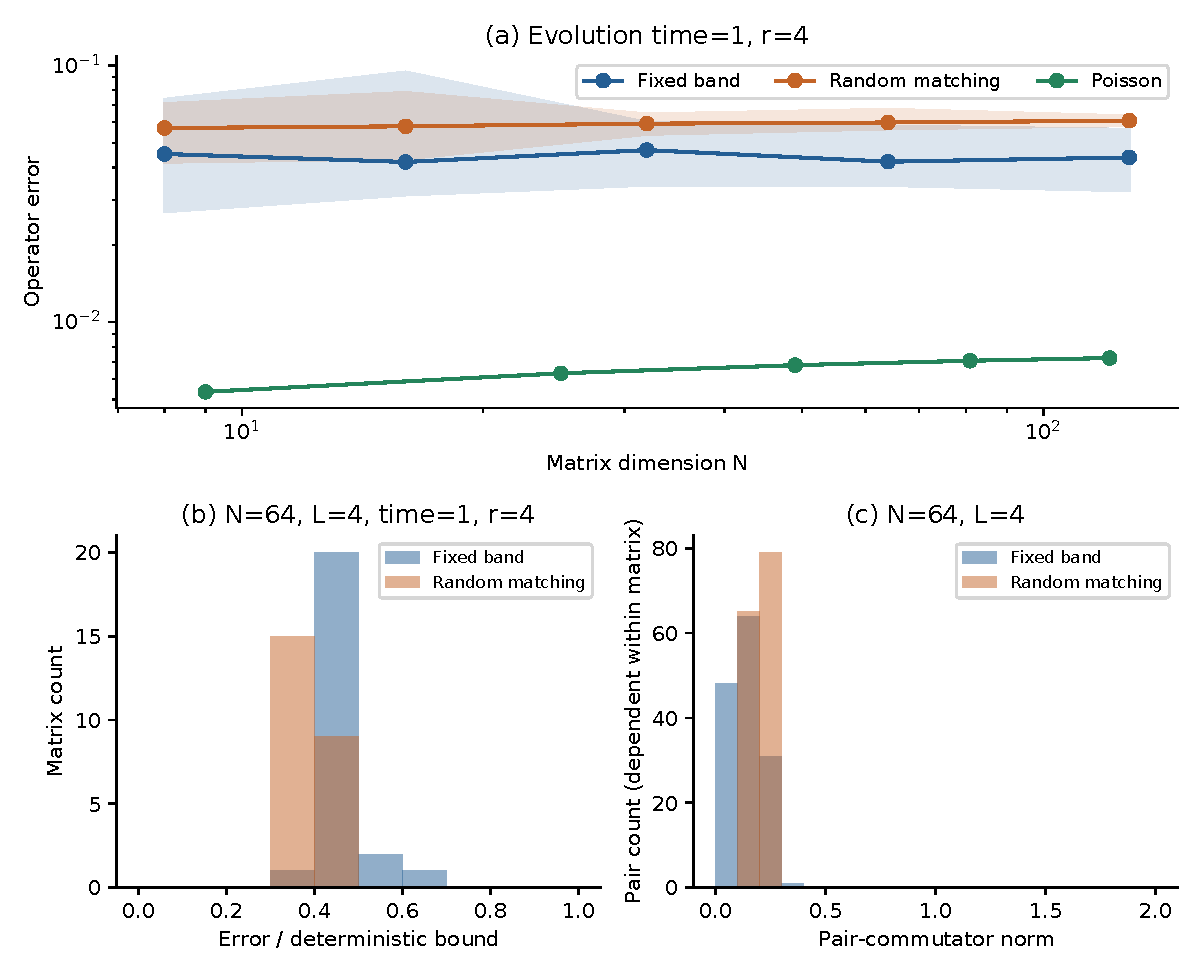
\includegraphics[width=\linewidth]{figures/overview.pdf}
\caption{Replacement for manuscript Figure 9. Top: median operator error versus $N$, at $\tau=1,r=4$, with four matching terms per synthetic matrix and the five-term Poisson decomposition. Bands show empirical 5th--95th percentiles; deterministic Poisson points have no sampling interval. Bottom left: error divided by $\tau^2\C/(2r)$ at $N=64,L=4,\tau=1,r=4$, 24 matrices per synthetic family. Bottom right: pair-commutator histograms for the same matrices, 144 pairs per family; pairs are clustered by matrix. Matrix laws, normalization and seeds are specified in the numerical protocol section. These plots illustrate finite-instance behavior, not proof by extrapolation.}
\label{fig:overview}
\end{figure}
\begin{figure}[p]
\centering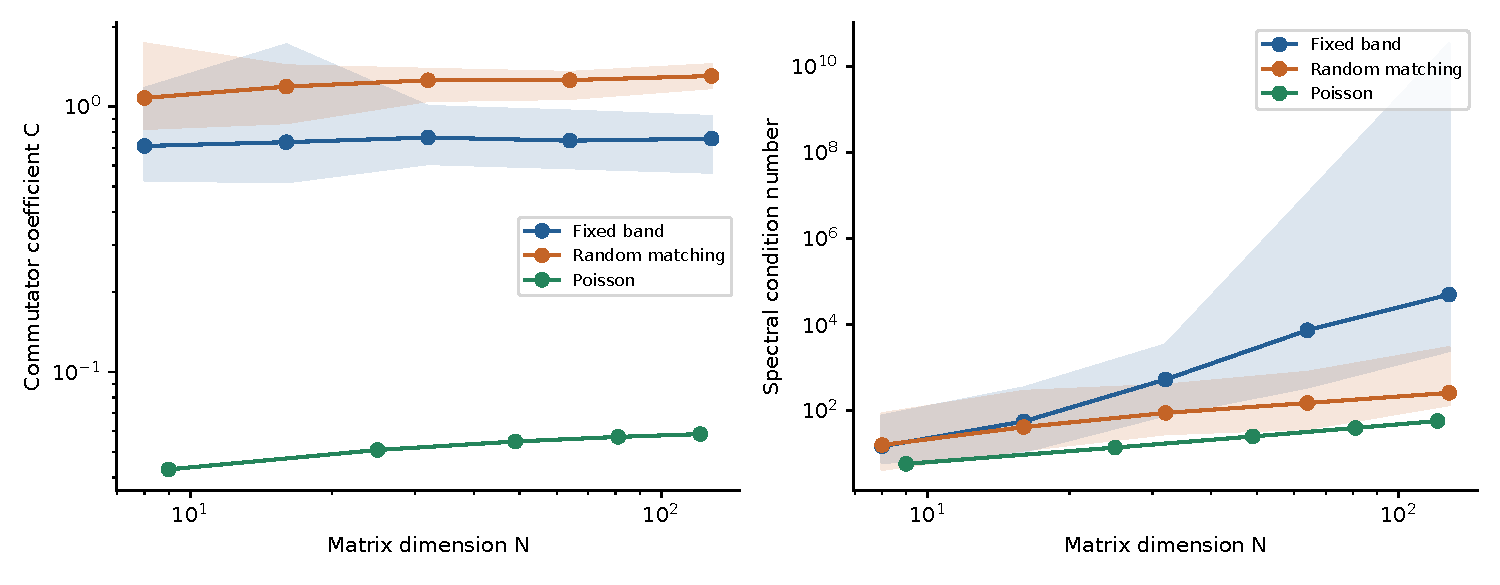
\includegraphics[width=\linewidth]{figures/family_parameters.pdf}
\caption{Parameters behind the error curves, using four matching terms for the synthetic families. Medians and empirical 5th--95th ranges are shown for 24 independent matrices at each size; Poisson points are deterministic. Synthetic conditioning is uncontrolled and can be much larger than the median. The Poisson coefficient stays bounded while its condition number grows. No statement that an indefinite synthetic matrix is an SPD application is implied.}
\label{fig:parameters}
\end{figure}

\begin{figure}[p]
\centering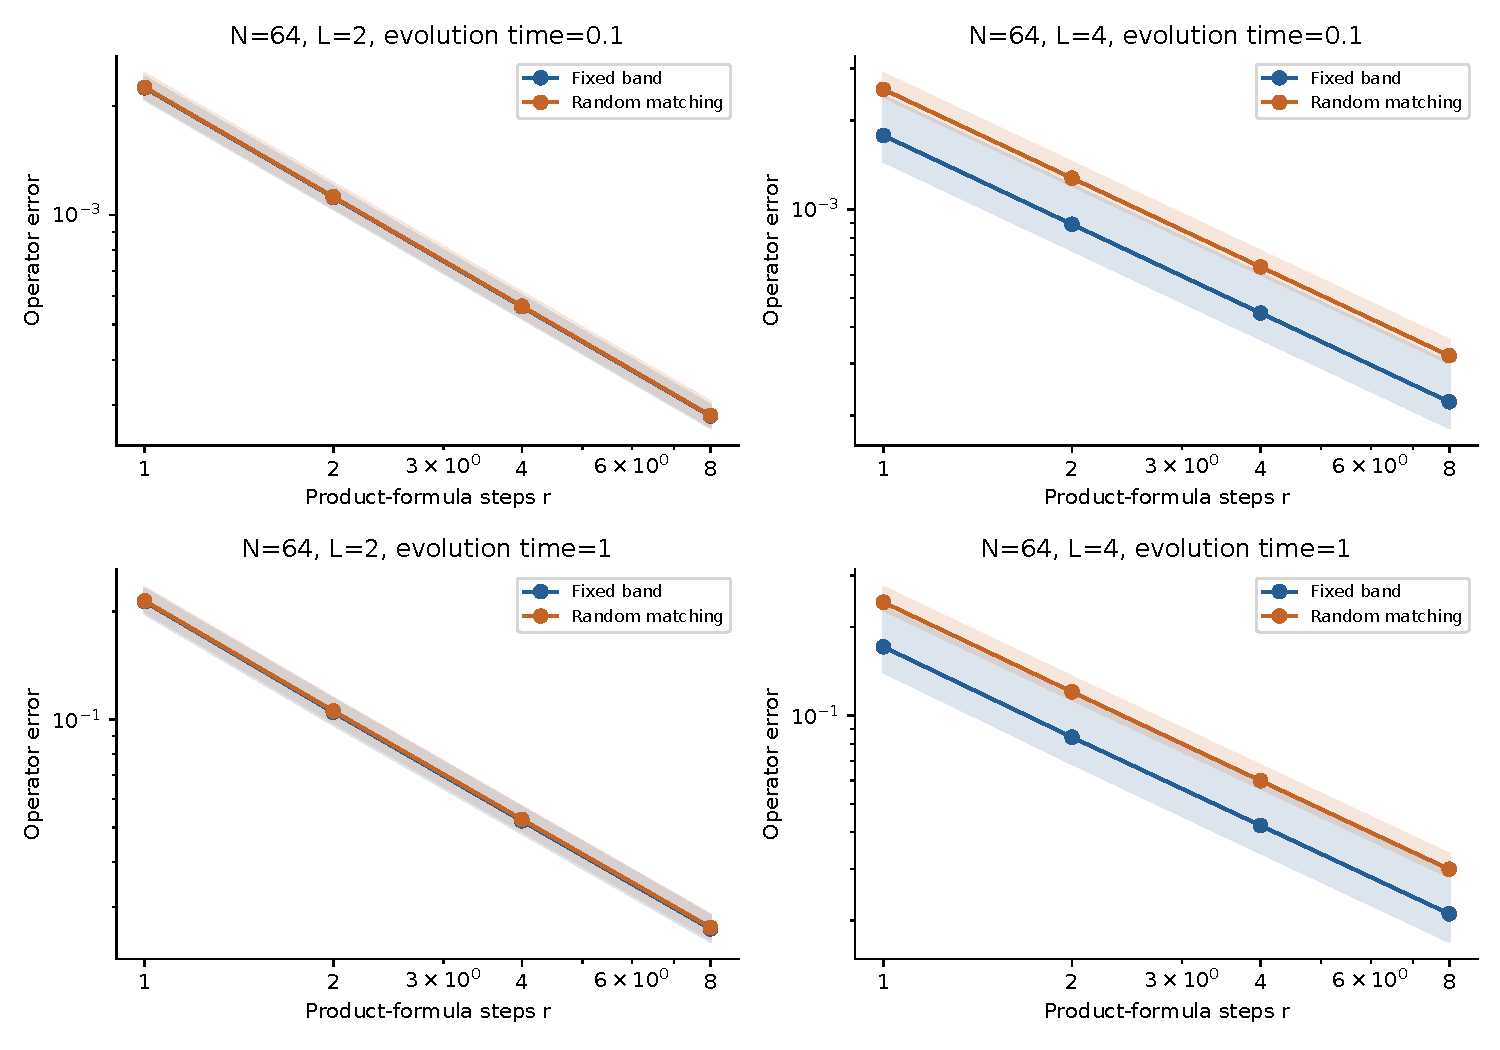
\includegraphics[width=\linewidth]{figures/step_sweeps.pdf}
\caption{Step-count sweeps at $N=64$ for both synthetic families, with $L=2$ or $4$ and $\tau=0.1$ or $1$. Each curve uses the same 24 matrices across $r=1,2,4,8$. Bands show empirical 5th--95th percentiles, not confidence bands or independent measurements across $r$. The observed decrease is consistent with the first-order guarantee; the proof, not a regression, determines the certified scaling.}
\label{fig:steps}
\end{figure}

\begin{figure}[p]
\centering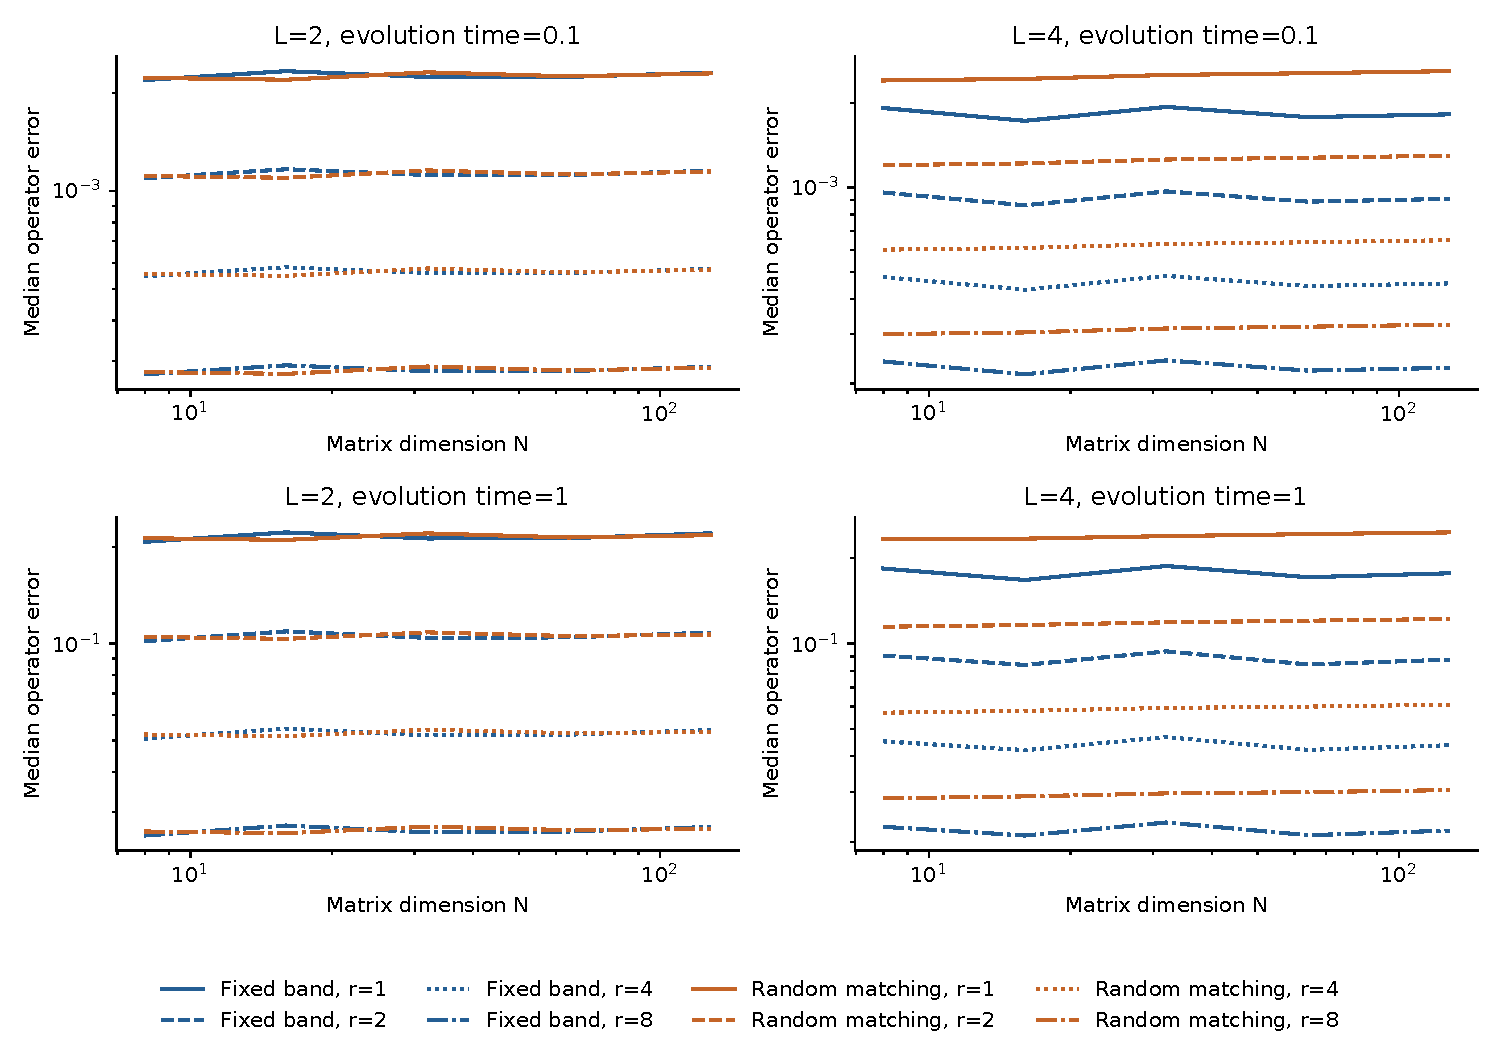
\includegraphics[width=\linewidth]{figures/all_configurations.pdf}
\caption{Median operator errors for every sampled synthetic parameter combination. Panels distinguish $L$ and $\tau$; colors distinguish the matrix family and line styles distinguish all four step counts. Every point summarizes 24 independent matrices. Uncertainty bands are omitted here for readability; Figure~\ref{fig:steps}, Figure~\ref{fig:overview}, Table~\ref{tab:ci}, and the archived summary give distribution information. This is a finite size sweep, not a fitted or extrapolated asymptotic law.}
\label{fig:all}
\end{figure}
\clearpage

\begin{table}[ht]
\centering\small\begin{tabular}{lrrrr}\toprule Family & $N$ & Mean error & 95\% mean CI & Max error\\\midrule
Fixed band & 8 & 0.04936 & [0.04164, 0.05855] & 0.12115\\
Fixed band & 16 & 0.05104 & [0.04305, 0.06005] & 0.10371\\
Fixed band & 32 & 0.04737 & [0.04380, 0.05099] & 0.06795\\
Fixed band & 64 & 0.04417 & [0.04065, 0.04806] & 0.07045\\
Fixed band & 128 & 0.04385 & [0.04073, 0.04725] & 0.06329\\
Random matching & 8 & 0.05690 & [0.05285, 0.06104] & 0.08142\\
Random matching & 16 & 0.05827 & [0.05417, 0.06249] & 0.07957\\
Random matching & 32 & 0.05949 & [0.05776, 0.06157] & 0.07611\\
Random matching & 64 & 0.06049 & [0.05884, 0.06238] & 0.07330\\
Random matching & 128 & 0.06108 & [0.06036, 0.06189] & 0.06772\\
\bottomrule\end{tabular}

\caption{Descriptive uncertainty at $L=4$, $\tau=1$, $r=4$. Each row uses 24 matrices; intervals are pointwise 95\% percentile-bootstrap intervals for the mean with 2,000 resamples. Maxima are observed maxima, not population bounds.}
\label{tab:ci}
\end{table}
The results do not show a universal equality between error and $\tau/r$, nor would a flat median establish one. Family, decomposition, conditioning and sample extrema carry distinct information. The two-dimensional PDE family has a provable bounded simulation coefficient for structural reasons, while its gap closes with increasing grid size.

\section{Tractable validation of HHL and discretization}
\subsection{Full successful-branch HHL test}
The exact-grid test takes
\begin{equation}
 H=0.5I+0.15Z+0.2X,\quad |b\rangle=(1,1)^T/\sqrt2,
 \quad m=3,\quad\tau_{\rm base}=2\pi.
\end{equation}
The eigenvalues are $0.25$ and $0.75$, with spectral condition number three. Three-bit QPE therefore occupies bins $k=2,6$. The reciprocal rotation uses $f(0)=0$ and $f(k)=\min\{1,0.25/(k/8)\}$ for $k>0$. On the occupied bins this is exactly $c/\lambda$, $c=0.25$.

The exact successful joint state has no clock leakage and equals the normalized dense solution. Its probability is $0.2$. This follows directly from
\[H^{-1}b=\frac{(0.15,0.45)^T}{0.1875\sqrt2},\qquad 0.25^2\norm{H^{-1}b}^2=0.2.\] The decomposition uses $0.5I$, $0.15Z$ and $0.2X$, so $\C=\norm{[0.15Z,0.2X]}=0.06$.

The approximate simulation replaces each of the three controlled powers with a first-order formula and uses its adjoint in inverse QPE. The test retains the whole successful clock/system state rather than projecting onto clock zero and silently renormalizing again. The conditional state errors and success probabilities are listed below.
\begin{table}[ht]
\centering\begin{tabular}{rrrr}\toprule $r$ & State error & Analytic bound & Success probability\\\midrule
16 & 0.03642488 & 2 & 0.2002979790\\
64 & 0.008801258 & 2 & 0.2000175474\\
256 & 0.002195571 & 0.8689711 & 0.2000010926\\
4096 & 0.0001372035 & 0.05431069 & 0.2000000043\\
\bottomrule\end{tabular}

\caption{Exact-grid HHL validation. The analytic state bound is capped at the maximum possible distance two for presentation; the archived uncapped values are also retained. The reference probability is $0.2$. This restricted exact-grid test does not establish a general finite-QPE/filter guarantee.}
\end{table}
\begin{figure}[ht]
\centering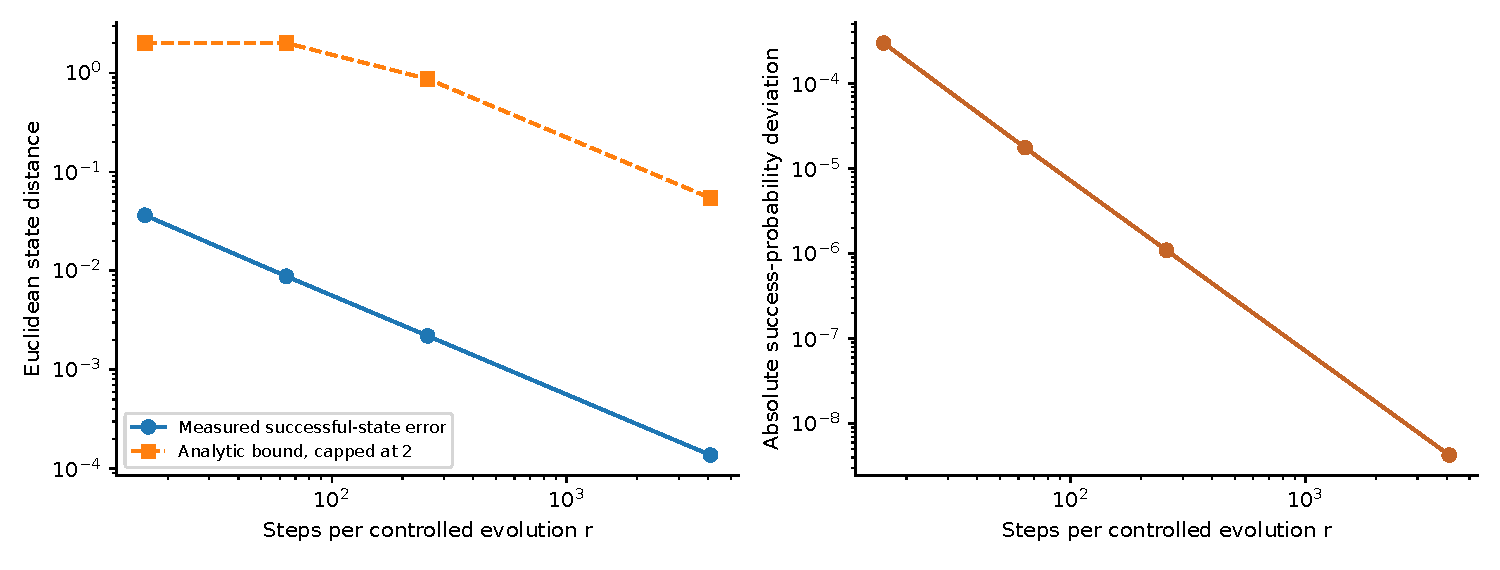
\includegraphics[width=\linewidth]{figures/hhl_validation.pdf}
\caption{HHL validation using the full successful clock/system branch. Left: measured state distance and the bound from equation~\eqref{eq:post}, capped at two. Right: absolute deviation of success probability from $0.2$. There is one deterministic circuit per step count, so no sampling interval is attached.}
\end{figure}
\clearpage

\subsection{Poisson checks}
\begin{table}[ht]
\centering\begin{tabular}{rrrr}\toprule $N$ & $\kappa_2$ & State error & Relative residual\\\midrule
9 & 5.828427 & 0.04006445 & 3.53e-16\\
25 & 13.9282 & 0.01592488 & 7.34e-16\\
49 & 25.27414 & 0.008624455 & 1.79e-15\\
81 & 39.86346 & 0.005424757 & 2.27e-15\\
121 & 57.69548 & 0.003732078 & 3.47e-15\\
\bottomrule\end{tabular}

\caption{Dense validation of the Poisson family and manufactured solution. The condition number agrees with the analytic spectrum to the test tolerance; residuals refer to the discrete solve and state errors to the normalized sampled continuum solution. Each row is deterministic.}
\end{table}
\begin{figure}[ht]
\centering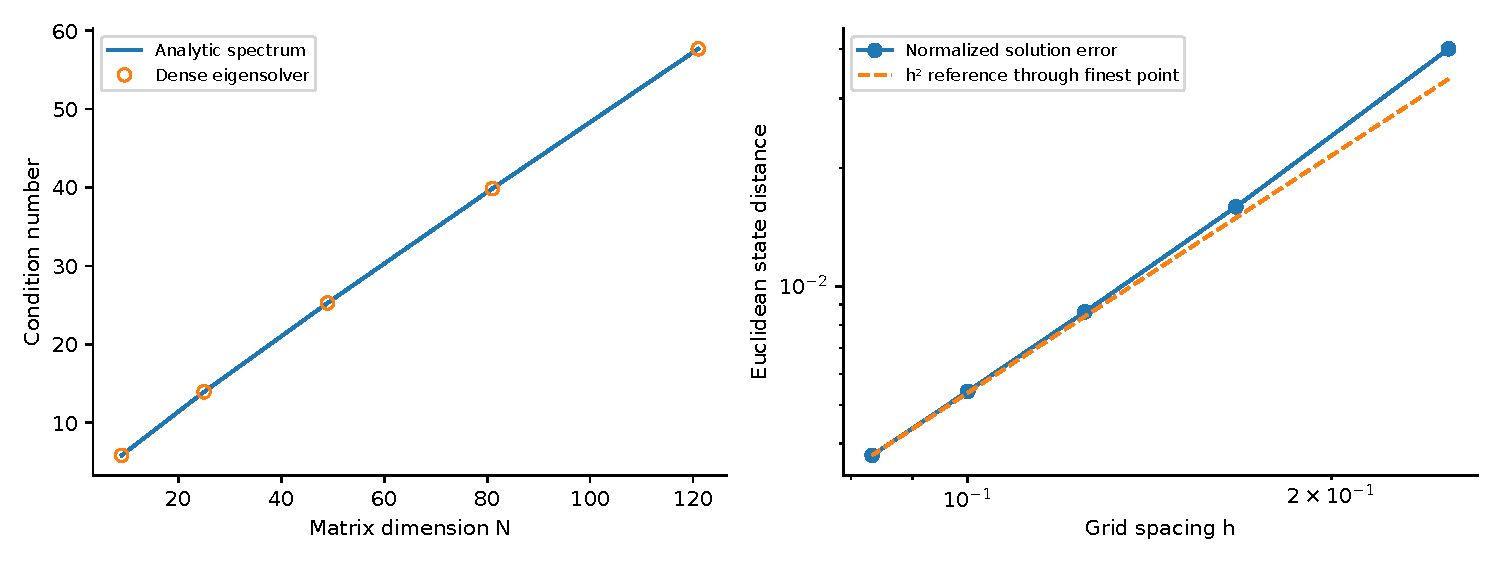
\includegraphics[width=\linewidth]{figures/pde_validation.pdf}
\caption{Poisson diagnostics. Left: dense condition numbers overlaid on equation~\eqref{eq:pdek}. Right: normalized discrete-versus-continuum solution error, with an $h^2$ reference passing through the finest-grid point. The reference is not fitted. Discretization bias and linear-solver residual are different quantities; a small residual does not eliminate discretization error.}
\end{figure}

\begin{figure}[ht]
\centering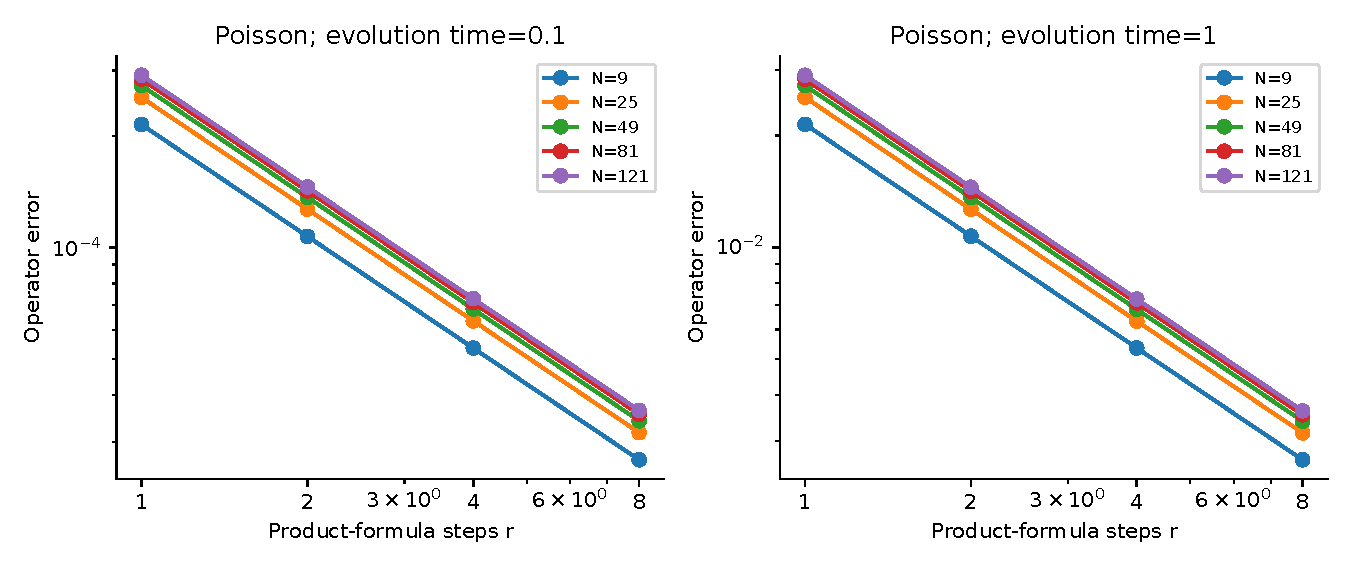
\includegraphics[width=\linewidth]{figures/pde_evolution_sweeps.pdf}
\caption{All deterministic Poisson evolution-error measurements: five sizes, two evolution times, and four step counts. Every curve uses the diagonal plus four parity matchings. These are simulation errors for the normalized discrete operator, distinct from the continuum discretization errors in the preceding figure. No sampling intervals apply.}
\end{figure}

\subsection{New validation of the completed theorem}
The added script \texttt{report/validate\_completed\_proof.py} uses seed 20260909. It checks 32 SPD decompositions at $N=2,4,8,16$, including commuting cases. For nonzero commutator bounds, the maximum measured effective-matrix error divided by $h\C$ is 0.4999303. Hermiticity of the principal effective matrix, the consistent-power identity for powers one, two and four, and the normalized inverse perturbation inequality pass the stated floating-point tests.

It also evaluates exact scalar QPE kernels and the binomial-order-statistic distribution of the median for 30 eigenphase configurations: $K\in\{4,8,12\}$, $\eps\in\{0.25,0.5\}$, and five eigenvalues per configuration. The largest single-register bad probability is 0.0248177, below $1/8$. Numerically evaluated median tails are at or below $1.2\times10^{-16}$, so their exact tiny values are limited by floating-point resolution; the analytic tail inequality, not those near-zero values, is the certificate. All reciprocal branch-error checks pass. These are lemma-level tests, not a simulation of the full coherent median circuit. Raw checks are attached as two CSV files with a JSON summary.

\subsection{Commuting and product-order regressions}
For commuting terms $Z,2Z$, the numerical product at $\tau=1,r=4$ agrees with $e^{3\ip Z}$ within $10^{-12}$. This checks the zero-commutator case independently of a nonzero bound.

The Q\# order-two coefficient routine currently returns ``halves + middle + halves'' rather than reversing the trailing halves. For three terms, the symmetric Strang sequence should be
\begin{equation}
 e^{\ip H_1t/2}e^{\ip H_2t/2}e^{\ip H_3t}
 e^{\ip H_2t/2}e^{\ip H_1t/2}.
\end{equation}
The existing ordering instead ends in $H_1/2,H_2/2$. Testing $H_1=Z$, $H_2=X$, $H_3=\operatorname{diag}(0.3,0.7)$, the local-error ratio $E(0.04)/E(0.02)$ is $7.9984111$ for the corrected symmetric sequence and $3.9989532$ for the existing sequence. These values are consistent with cubic versus quadratic local error. They diagnose a coefficient-order issue; no compiled Q\# correctness test was run. The first-order theorem here does not depend on the order-two routine.

\section{Logical interface, example schedule, and implications}
\subsection{A concrete sufficient schedule}
For the exact-grid instance above, take a conservative reference lower bound $p_{\min}=1/9$ and PF state budget $0.01$. Then $\eta_{\rm target}=1/600$, and the allocation~\eqref{eq:schedule} gives
\begin{equation}
 (r_0,r_1,r_2)=(9949,19898,39795),\qquad\HS=417852.
\end{equation}
The resulting full-circuit PF bound is $0.0016666171$; the conditioned PF bound is $0.0099997026$. The PF-only success lower bound is $0.1100028107$, giving a diagnostic expected-attempt upper bound $9.0906768$. These are sufficient schedule outputs, not measured optimal invocation counts. The reference's exact success is $0.2$ and the analytic lower bound is deliberately conservative. Other implementation errors must be added before a final retry cap is certified.

\subsection{Task 01 contract and counting ownership}
The archived adapter in this subsection describes the earlier direct-unitary schedule, not the median-QPE circuit of Theorem~\ref{thm:complete}. Its example count 417852 must not be assigned to the new theorem. The exported \texttt{contract-stage.json} satisfies the stage definition of Task 01's version 1.0.0 schema. It is a stage fragment, not a complete evaluated workload. It covers \texttt{q.core}, with multiplicity one, and contains forward QPE, the reciprocal and inverse QPE. Preparation, heralding measurement, readout, classical setup and QEC/hardware resources are outside that coverage. Task 05 must incorporate the core once into an attempted circuit and apply external repetitions exactly once.

Original matrix parameters belong in \texttt{pp.N}, \texttt{pp.s\_row}, \texttt{pp.s\_col}, and \texttt{pp.kappa\_2}. Parameters of the normalized or effective operator, including $L$, $\C$, $\tau_{\rm base}$, $m$ and $p_{\min}$, together with state budgets belong in the quantum configuration; they must not overwrite original conditioning or the common output tolerance. Counts carry units of gates, queries, layers or logical qubits; unknown compilation quantities remain unknown or symbolic, not zero.

For the example, an exclusive compiled gate bucket $g$ is exported as $417852\,g_{\rm HS1}+g_{\rm nonHS}$. Oracle queries remain unexpanded. T-depth, dependency depth and workspace remain symbolic pending actual implementations. Schema validity does not certify a QPE approximation, a success bound for arbitrary inputs, or a physically complete cost model.

For a Hermitian observable $O$ of norm at most one and unit vectors $x,y$,
\begin{align}
 |\langle x,Ox\rangle-\langle y,Oy\rangle|
 &\leq|\langle x-y,Ox\rangle|+|\langle y,O(x-y)\rangle|\\
 &\leq2\norm{x-y}.
\end{align}
This gives a conservative conversion from vector error to that particular observable error. A different physical functional, norm recovery or relative-error target needs a different declared conversion. Discretization, algorithmic bias and stochastic failure are not interchangeable budgets.

\subsection{Consequences for the manuscript and downstream estimates}
The unsupported B19 and its use in B28/Proposition 1 must be replaced by the conditional bounds here. The corresponding estimator expression in \texttt{tools/surface\_code\_opt.py} cannot remain a certified cost input. A change in invocation count requires new compiled gate/depth/workspace inputs, then new QEC scheduling and hardware calculations; it cannot be translated into seconds or joules by one universal multiplier.

The original $2^{33}$--$2^{48}$ crossover range and associated $10^5$ physical-qubit, $10^6$-second, and $10^{12}$--$10^{13}$-joule statements should not be carried into the revised analysis as validated estimates without recomputation. A conservative upper bound does not determine the actual optimized crossover shift or rule out an advantage.

The remaining practical inputs are the final application generator and output/error contract, its input and access model, its preconditioner, compiled module costs and full I/O accounting. Theorem~\ref{thm:complete} now certifies QPE and filter accuracy for its stated construction; a different QPE implementation would require a separate certificate. The Poisson example establishes $s\leq5$ and $\kappa_2=\Theta(N)$ for a specific unpreconditioned family; it does not complete that missing application contract. Shared repository source has not been modified as part of this report.

\appendix
\section{Original numerical inference and implementation audit}
The review calls the main result ``Statement 1''; the supplied manuscript labels it Proposition 1 on page 3. Its Figure 9 is on page 18, although a minor review comment calls it ``Fig. 19, pg. 17.'' These refer to the same unlabeled-distribution concern.

\subsection{Recovered historical notebook settings}
Embedded MATLAB XML in \texttt{num/distributions.mlx} specifies 1,000 one-sparse matrices at dimension 16, zero-probability parameter 0.2, and all 499,500 pair commutators. Those pair samples are dependent. A second loop specifies 10,000 matrices at inherited dimension 16, $s=\lfloor\log(16)\rfloor=2$, $6s^2$ generator slots, $\tau=0.1,r=1$, and the effective-log diagnostic \texttt{epsA}.

\texttt{num/trotterErrorAnalysis.mlx} contains different experiments: dimensions 4 and 8 with $r=1{:}20$ and one matrix per size; a size sweep $2{:}128$ with one matrix per size; ten dimension-32 matrices over times 0.01--0.2; and a separate 10,000-sample unitary-error histogram at dimension 16, $s=3$, $\tau=0.1,r=1$. These use different error observables and do not establish uniform-in-size behavior. Historical seeds and raw samples are not archived, so the exact displayed histograms have not been reconstructed.

\subsection{Code findings relevant to scaling}
\begin{longtable}{p{.32\linewidth}p{.60\linewidth}}
\toprule Location & Finding and consequence \\\midrule\endhead
\texttt{num/genSparse.m} & Reseeds with wall-clock shuffle inside every term; duplicates diagonal sparse insertions; counter tests \texttt{p\ ~=\ 1} rather than comparison with the selected partner. Zero choices can revisit unchanged vertices. The old law should not be described as uniform sampling of sparse matrices.\\[5pt]
\texttt{num/epsA.m} & Uses principal \texttt{logm} without phase-branch certification and compares complex unitary eigenvalues with zero. Returned error is absolute, although some notebook axes say relative error.\\[5pt]
\texttt{num/trotter.m} & Implements the first-order ordered dense exponential product and matrix power. It includes no access, synthesis or QEC cost.\\[5pt]
\texttt{num/hhl.m} & Uses dense GPU exponentials and extracts clock-zero amplitudes after uncomputation before another normalization, without reporting that projection probability or full clock leakage.\\[5pt]
\texttt{TrotterSuzuki.qs} & Order-two trailing half-list is not reversed; the tractable validation section reports a finite regression demonstrating the lost local order for a three-term instance.\\[5pt]
\texttt{HamiltonianSimulation.qs} & Enumerates $6s^2$ color coefficients and hard-codes first order with two repetitions; this is not the derived accuracy-driven schedule.\\[5pt]
\texttt{HHL.qs} & Clock width and precision are fixed, a Trotter parameter is unused, a sparse call passes sparsity two, and the general repeat-until-success loop is commented out.\\[5pt]
\texttt{PhaseEstimation.qs} & Controlled powers are $2^j$; inverse QPE is induced by the enclosing construction and must also be counted.\\[5pt]
\texttt{Oracle.qs} & Traverses dense supplied arrays and emits controlled position/value table entries for nonzeros. This is not evidence for a size-independent lookup circuit.\\[5pt]
\texttt{surface\_code\_opt.py} & The HHL class implements the old prefactor and multiplies $18n+90b_{\rm bits}+15$. Its fixed ancilla field is not included in the peak estimate. Downstream notebooks inherit these inputs.\\
\bottomrule
\end{longtable}
These findings motivate integration fixes and compiled validation, not a claim that the Q\# implementation has been repaired in this task. The new dense experiments use seeded generators and the proved first-order formula independently.

\section{Reproduction and artifact inventory}
The archived experimental inputs use repository commit
\begin{center}\texttt{66a01648db95465abbd2f099d9b8f103679555b6}.\end{center}
Per-file SHA-256 hashes, rather than the commit alone, record the exact inspected working-tree inputs. The results directory is
\begin{center}\texttt{paper-revise/results/03-hhl-analysis/}.\end{center}
\begin{itemize}
\item \texttt{experiments.py}: seeded ensembles, dense error measurements, bootstrap summaries, original replacement Figure 9, and tractable validation.
\item \texttt{validate\_pde.py}: analytic-spectrum and manufactured-solution checks.
\item \texttt{samples.csv}, \texttt{commutators.csv}, \texttt{summary.csv}: raw and summarized simulation measurements.
\item \texttt{validation.json}, \texttt{pde-validation.csv}: deterministic validation results.
\item \texttt{logical\_model.py}, \texttt{model-input.json}, \texttt{model-output.json}: schedule helper and the concrete example.
\item \texttt{export\_contract.py}, \texttt{contract-stage.json}, \texttt{contract-validation.json}: Task 01 stage export and structural validation.
\item \texttt{manifest.json}, \texttt{input-versions.json}, \texttt{requirements-tested.txt}: input and environment provenance.
\item \texttt{report/completed-theorem.tex}: the completed theorem.
\item \texttt{report/validate\_completed\_proof.py}: new lemma-level checks.
\item \texttt{report/completed\_schedule.py}: exact integer schedule for the new theorem, separate from the earlier direct-unitary adapter.
\item \texttt{report/make\_figures.py}: generates the additional report figures and numerical tables from archived CSV/JSON files, without rerunning experiments.
\item \texttt{report/hhl-logical-scaling.tex}: editable source for this report.
\end{itemize}
To regenerate measurements, in the results directory and a compatible Python environment, run
\begin{verbatim}
export OPENBLAS_NUM_THREADS=1
export OMP_NUM_THREADS=1
python experiments.py
python validate_pde.py
python logical_model.py model-input.json > model-output.json
python export_contract.py
\end{verbatim}
To rebuild the report from those archived results, run the supplied report build script. The report build uses Tectonic 0.17.0 and the numerical plotting environment; a separate PyMuPDF environment is used only for final PDF validation and embedded reproducibility attachments. Modern package versions can produce slightly different floating-point/plotting results and should be recorded when rerunning.

The single distributed PDF also contains attachments with the raw measurements, numerical scripts, manifests, and report source. Attachment support depends on the viewer; the report text, derivations, captions and numerical conclusions are readable without opening them. No MATLAB execution, Q\# compilation, QEC simulation or physical crossover validation is claimed.

\begin{thebibliography}{9}
\bibitem{trotter} A.~M.~Childs, Y.~Su, M.~C.~Tran, N.~Wiebe, and S.~Zhu,
\emph{Theory of Trotter Error with Commutator Scaling}, Physical Review X \textbf{11}, 011020 (2021).
\href{https://doi.org/10.1103/PhysRevX.11.011020}{doi:10.1103/PhysRevX.11.011020};
\href{https://arxiv.org/html/1912.08854v3}{arXiv:1912.08854v3}, Section 5.1, Proposition 15, equations (143)--(145). Primary source verified 8 September 2026.
\bibitem{hhl} A.~W.~Harrow, A.~Hassidim, and S.~Lloyd,
\emph{Quantum algorithm for solving linear systems of equations}, Physical Review Letters \textbf{103}, 150502 (2009).
\href{https://arxiv.org/abs/0811.3171}{arXiv:0811.3171};
\href{https://doi.org/10.1103/PhysRevLett.103.150502}{doi:10.1103/PhysRevLett.103.150502}. Primary record verified 8 September 2026.
\bibitem{synthesis} P.~Selinger, \emph{Efficient Clifford+T approximation of single-qubit operators}, \href{https://arxiv.org/abs/1212.6253}{arXiv:1212.6253}. Primary record checked 9 September 2026. Rotation compilation is a separate cost and precision layer; no original module prefactor is inferred from this reference.
\bibitem{manuscript} Y.~Tu et al.,
\emph{Towards identifying possible fault-tolerant advantage of quantum linear system algorithms in terms of space, time and energy},
\href{https://arxiv.org/abs/2502.11239v2}{arXiv:2502.11239v2} (2025).
The locally supplied manuscript PDF is authoritative for the equation/page audit and is hash-recorded; its binary is not assumed identical to the public version.
\end{thebibliography}
\end{document}
